% /D:/UNIPA/ASD/notazione asintotica.tex
% A very simple LaTeX page to learn basic markup

\documentclass[11pt]{article}
\usepackage[utf8]{inputenc}
\usepackage[T1]{fontenc}
\usepackage{amsmath,amssymb,amsthm}
\usepackage{graphicx}
\usepackage{hyperref}
\usepackage[export]{adjustbox}

\graphicspath{{../imgs/}}

\title{Crescita delle funzioni}
\author{Riccardo Di Michele}
\date{}

\newtheorem{theorem}{Theorem}

\begin{document}
\maketitle

\section*{Crescita del costo computazionale}
Abbiamo già visto come calcolare \textbf{il tempo di esecuzione} di un algoritmo, per esempio,
l'algoritmo \emph{insertion sort} ha come costo computazionale: 
\[ f(n) = an^2 +bn +c \]

Ma spesso avremmo bisogno di informazioni in più.
Vogliamo sapere quanto questo tempo \textbf{cresce} all'aumentare dell'input. \\
Prendendo come esempio il costo analizzato prima proviamo a fare un calcolo matematico:
proviamo a vedere come si comporta quel costo per \emph{n molto grandi}, proviamo quindi
a calcolare il suo \textbf{limite}.
\[
  \lim_{n \to \infty}{an^2 +bn +c} \longrightarrow 
  \lim_{n \to \infty}{n^2 + n} \longrightarrow 
  \lim_{n \to \infty}{n^2}
\]

Poichè siamo di fronte a un limite, valori come i coefficienti diventano insignificanti
per $n \to \infty$ e il termine $n^2$ invece "domina" sui termini di grado inferiore.
Diremo quindi che l'algoritmo di \emph{insertion sort}, per un input sempre più grande,
crescerà \emph{come} $n^2$, oppure, in maniera più corretta, diremmo $\Theta(n^2)$, 
\emph{"theta grande di $n^2$"}. \\
Introduciamo allora il concetto della \textbf{notazione asintotica},
ovvero definire i \emph{limiti} di crescita di un certo costo per input sempre
più grandi. I vari tipi di notazione (vedremo nel dettaglio dopo) servono a dichiarare
il \textbf{\emph{lower bound}} e l'\textbf{\emph{upper bound}}, che corrispondono al
\emph{limite inferiore} e al \emph{limite superiore} della nostra funzione.
L'\emph{upper bound} sarà indicato da $O(g(n))$, da leggere come \emph{"O grande di $g(n)$"}, mentre
il \emph{lower bound} da $\Omega(g(n))$, letto come \emph{"Omega grande di $g(n)$"}. \\
Una nota importante: nonostante esistano diverse notazioni dobbiamo sottolineare il fatto che
sono solo e soltanto delle \underline{nomenclature}: quando leggiamo $\Theta(n)$ oppure 
$\Omega(n^2)$ è solo un modo per descrivere l'andamento di una funzione al crescere di n,
non dobbiamo leggere queste notazioni come "\emph{a $n^2$ applico la proprietà $\Omega$}".

\subsection*{Caso peggiore e caso migliore}
Dobbiamo prima però fare una distinzione molto importante tra i \emph{\textbf{casi dell'algoritmo}}.
Prendiamo come esempio il seguente algoritmo per calcolare una potenza \emph{ennesima} di $2$.

\begin{verbatim}
  function power_2(n)
    f = 1
    for i = 1 to n do
      f = f * 2
    end for

    return f
\end{verbatim}

In questo caso il costo dell'algoritmo è \textbf{fisso} poichè farà sempre
$n$ cicli.\newline
Troveremo però algoritmi il cui numero di cicli (e costo) non sarà fisso, per esempio
l'algoritmo di \emph{\textbf{binary search}}.

\begin{verbatim}
  function binary_search(A, n, T)
    L = 0
    R = n - 1
    while L <= R do
      m = L + floor((R - L) / 2)
      if A[m] < T then
        L = m + 1
      else if A[m] > T then
        R = m - 1
      else
        return m
    return unsuccessful
\end{verbatim}

È importante notare che, a differenza del primo algoritmo, questo 
presenta un \emph{if statement} capace di far terminare l'algoritmo in qualsiasi
momento. Questo rende impossibile stabilire un numero finito di cicli, quindi, dovremmo studiare
l'algoritmo a seconda del \textbf{\emph{caso migliore}} (minor numero di cicli) 
e \textbf{\emph{caso peggiore}} (maggior numero di cicli). \\
Facendo un esempio con l'algoritmo sopra citato il \emph{caso migliore} sarebbe quando
$A[m]$ coincide con $T$ al primo ciclo, avendo un costo computazionale pari a $f(n) = 1$;
il \emph{caso peggiore} sarebbe invece quando l'algoritmo non trova l'elemento $T$, e 
avremmo così un costo di $f(n) = log_2 (n) +1$.
Una volta che abbiamo chiaro questi concetti possiamo continuare spiegando
i tipi di \emph{notazioni asintotiche}.

\subsection*{Notazione asintotica $\Theta$}
Formalmente diremmo che
\[
  \Theta(g(n)) = f(n) \iff
  \exists \hspace{4px} c_1, c_2, > 0,
  \hspace{4px} n_0 > 0 
  \mid 
  c_1 \cdot g(n) \le f(n) \le c_2 \cdot g(n)
  \hspace{4px} \forall n \ge n_0
\]

\begin{figure}[t]
  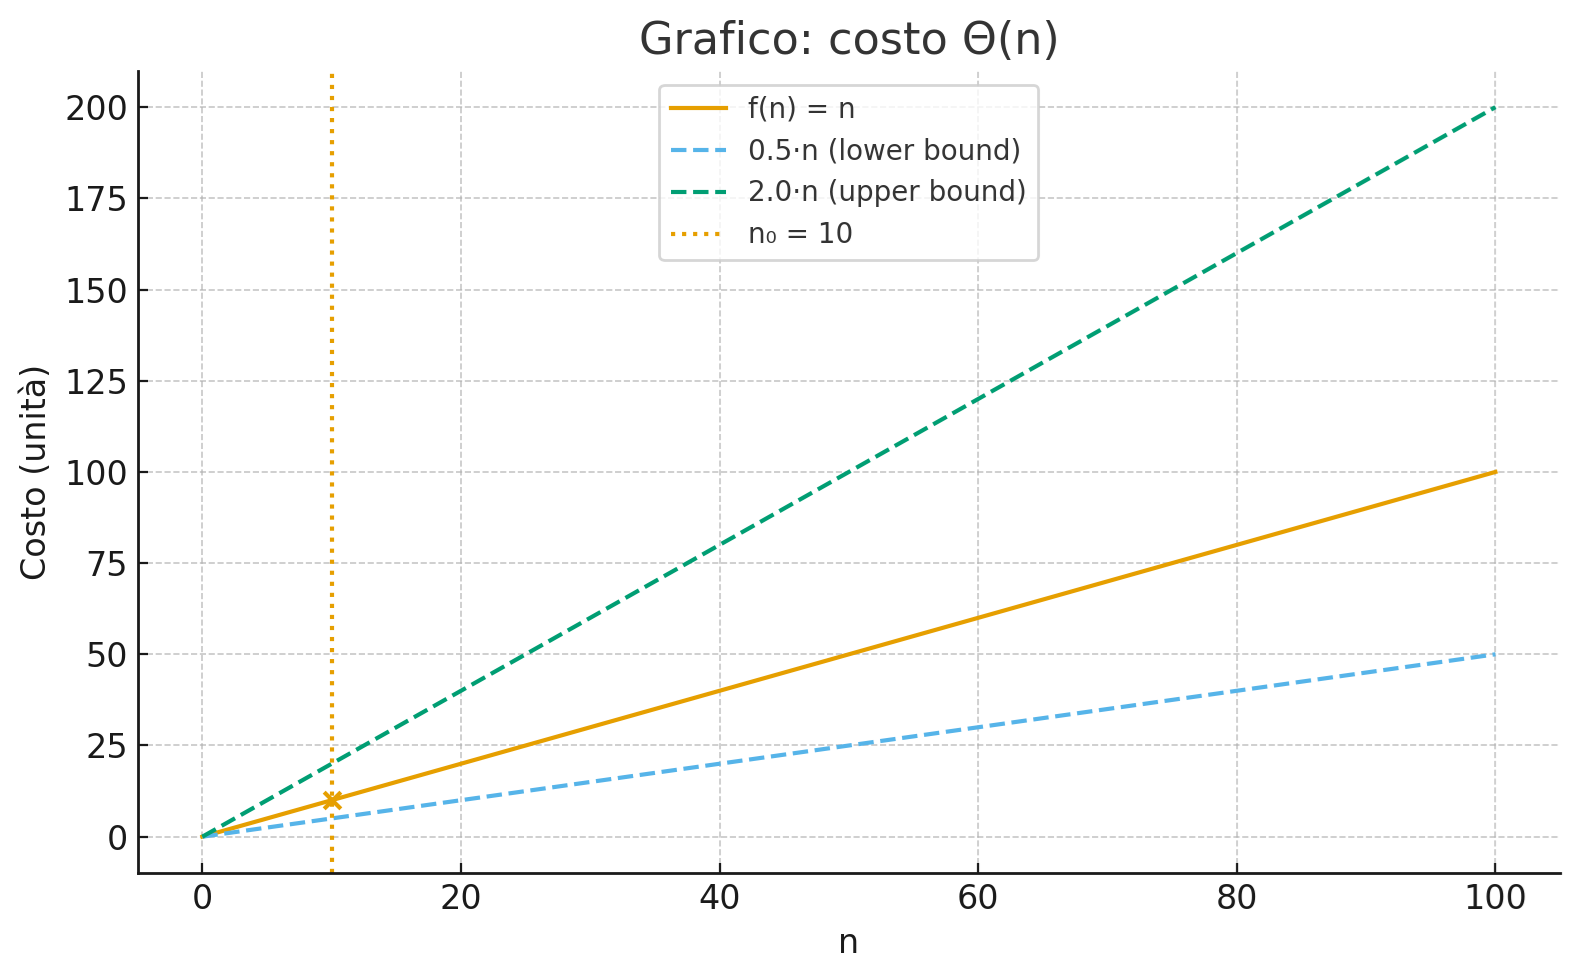
\includegraphics[scale=0.16, center]{theta_placeholder.png}
\end{figure}

dopo un certo indice $n_0$ il nostro \emph{costo computazionale} $f(n)$ sarà compreso
dentro una curva che avrà $c_1 \cdot g(n)$ come limite superiore e $c_2 \cdot g(n)$
come limite inferiore.
Poichè $c_1$ e $c_2$ possono essere qualsiasi valore positivo troveremo più di una funzione del tipo
$c \cdot g(n)$ che soddisfa la proprietà enunciata, diremo infatti che $\Theta(g(n))$ è
un'insieme di queste funzioni; proprio per questo motivo sarebbe più corretto scrivere 
$f(n) \in \Theta(g(n))$ ma la notazione $f(n) = \Theta(g(n))$ ha lo stesso valore. \\

L'algoritmo preso in figura è il \textbf{power\_2} analizzato nel paragrafo prima e
possiamo notare, come detto poc'anzi, che in realtà esistono altri possibili lower bound e 
upper bound; in parole povere potevamo anche prendere un "intervallo" più piccolo.

\subsection*{Notazione asintotica $O$}
Abbiamo già parlato di come la \emph{notazione $\Theta$} limita una funzione sia superiormente che
inferiormente, ma spesso ci sarà possibile indicare solo il limite superiore,
in quel caso useremo la notazione $O$.
\[
  O(g(n)) = f(n) \iff
  \exists \hspace{4px} c > 0, n_0 > 0 \mid
  0 \le f(n) \le c \cdot g(n) \hspace{4px}
  \forall \hspace{4px} n \ge n_0
\]

\begin{center}
  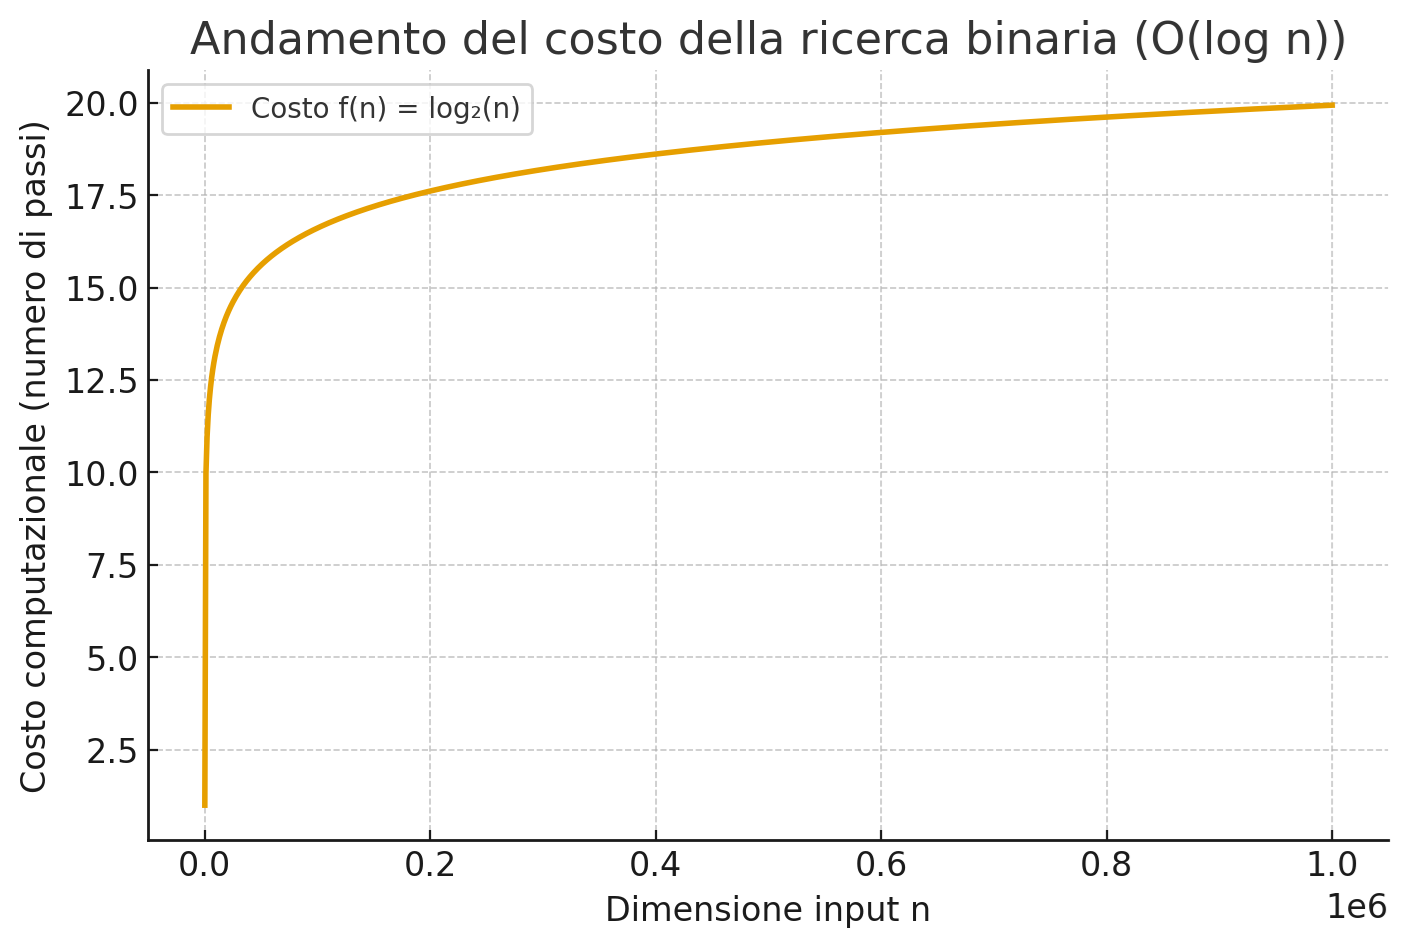
\includegraphics[scale=0.16]{O_placeholder.png}
\end{center}

per tutti i valori a "\emph{destra}" di $n_0$ i valori di $f(n)$ coincidono
o si trovano sopra $c \cdot g(n)$. \\
Ovviamente una funzione che appartiene già a un insieme $\Theta(g(n))$ sarà
anche appartenente all'insieme $O(g(n))$, poichè una funzione in $\Theta$ è munita
sia di limite superiore che inferiore; possiamo quindi dire che l'insieme
$\Theta \subseteq O$. \\

L'algoritmo in figura questa volta è il \emph{binary search} un algoritmo dove
non possiamo calcolare un numero fisso di cicli poichè al suo interno vi sono 
presenti degli \emph{if statement} che possono far terminare l'algoritmo,
di conseguenza ci limiteremo a calcolare il suo costo nel caso peggiore, ovvero 
$log_2 (n)$. \\
Diremo allora che $f(n) = O(log_2 (n))$.

\subsection*{Notazione asintotica $\Omega$}
Ovviamente, la notazione $\Omega$ indicherà invece un limite inferiore di una certa funzione;
formalmente diremo
\[
  \Omega(g(n)) = f(n) \iff
  \exists \hspace{4px} c > 0, n_0 > 0 \mid
  0 \le c \cdot g(n) \le f(n) \hspace{4px}
  \forall \hspace{4px} n \ge n_0
\]
\begin{center}
  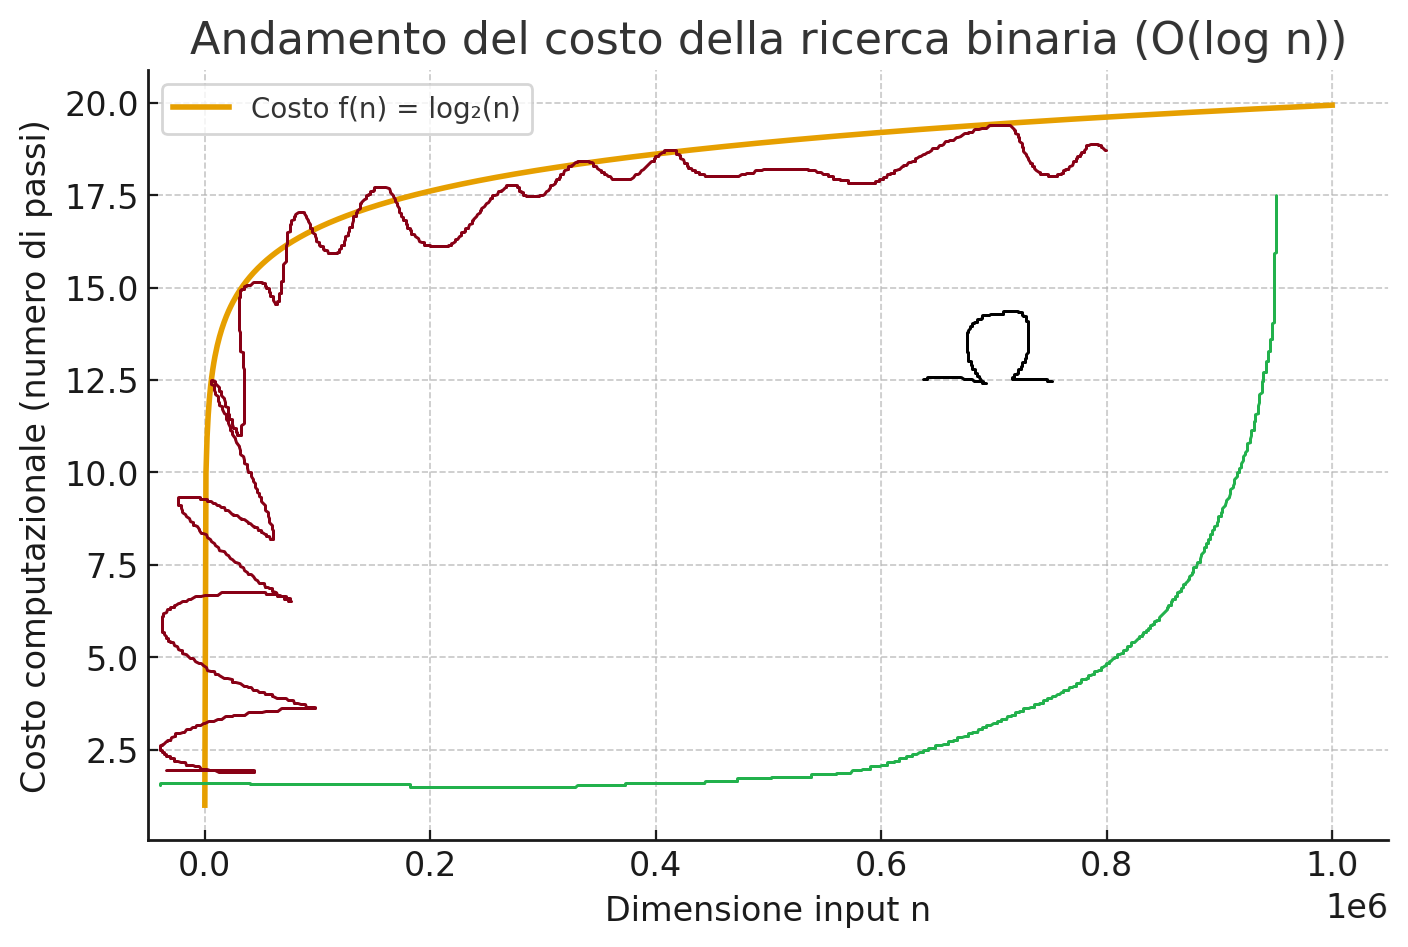
\includegraphics[scale = 0.16]{Omega_placeholder.png}
\end{center}

per tutti i valori a "\emph{destra}" di $n_0$ i valori di $f(n)$ coincidono
o si trovano sopra $c \cdot g(n)$.
\\

Questo è l'algoritmo del pisello duro e mi serve questo paragrafo
solo come placeholder ciao haha lol

\subsection*{Proprietà principale delle notazioni asintotiche}


\end{document}